\documentclass[12pt]{article}
\usepackage{ctex}
\usepackage[english]{babel}
\usepackage{amsfonts}
\usepackage{makecell}
\usepackage{graphics}
\usepackage{graphicx}
\usepackage{fancyhdr}
\usepackage{ifthen}
\usepackage{wrapfig}
\usepackage{array}
\usepackage{colortbl}
\usepackage{fullpage}
\usepackage[table]{xcolor}
\usepackage{subfigure}
\usepackage{caption}
\usepackage{float}
\usepackage{ctex}
\usepackage{appendix}
\usepackage{shorttoc}
\usepackage{pagenote}
\usepackage{setspace}
\usepackage{geometry}
\usepackage{indentfirst}
\usepackage{fullpage}
\usepackage{booktabs}
\usepackage{multirow}
\usepackage{longtable}
\usepackage{minipage-marginpar}
\usepackage{hyperref}
\usepackage{palatino}
\usepackage{setspace}
\usepackage{subfigure}
\usepackage{picinpar}
\usepackage{newtxtext}
\usepackage{amsmath,amssymb,amsthm}
\usepackage{extarrows}
\usepackage{algorithm}
\usepackage{algorithmic}
\usepackage{paralist}
\usepackage{newtxmath} % must come after amsXXX
\usepackage{lastpage}
\usepackage{clrscode3e}
%\RequirePackage{graphics}
% Replace ABCDEF in the next line with your chosen problem
% and replace 111111 with your Team Control Number
% and replace abcdef with your Title
% and replace 123456 with the number of pages of your essay
\newcommand{\Problem}{A}
\newcommand{\Team}{{2226594}}
\newcommand{\Title}{{Power Profile of a Cyclist}}
\newcommand{\wholepages}{\pageref{LastPage}}
\newcommand{\itembf}{\item \textbf}
\title{\Huge\textbf{\Title}}
\author{Team\#\Team}
\date{\today}

%%%%%%%%%%%%%%%%%%%%%%%%%%%%%%%%%%%%%%%%
% set up of theorems

\newtheorem{thm}{Theorem}[section]
\newtheorem{cor}[thm]{Corollary}
\newtheorem{lem}[thm]{Lemma}
\newtheorem{prop}[thm]{Proposition}
\theoremstyle{definition}
\newtheorem{defn}[thm]{Definition}
\theoremstyle{remark}
\newtheorem{rem}[thm]{Remark}
\numberwithin{equation}{section}
\newtheorem{theorem}{Theorem}
\newtheorem{corollary}[theorem]{Corollary}
\newtheorem{lemma}[theorem]{Lemma}
\newtheorem{definition}{Definition}

%%%%%%%%%%%%%%%%%%%%%%%%%%%%%%%%%%%%%%%%
% setup of page length and script size

\setlength{\belowcaptionskip}{4pt}
\setlength{\abovecaptionskip}{5pt}
\setlength{\headsep}{0.4in}
\setlength{\headheight}{14.5pt}
\captionsetup{font={footnotesize}}
\renewcommand{\baselinestretch}{1}
\setlength{\parskip}{0.28em}
\geometry{bottom=1in}



%%%%%%%%%%%%%%%%%%%%%%%%%%%%%%%%%%%%%%%%
% set up of page style

\pagestyle{fancy}
\fancyhead[L]{Team\ \#\Team}
\fancyhead[C]{\Title}
\fancyhead[R]{Page \thepage \ of \wholepages}
\fancyfoot{}

%%%%%%%%%%%%%%%%%%%%%%%%%%%%%%%%%%%%%%%%
% hyphenation

\tolerance=1
\emergencystretch=\maxdimen
\hyphenpenalty=10000
\hbadness=10000

\hypersetup{hidelinks} 
\hypersetup{
	colorlinks=false,
	linkcolor=black,
	citecolor=black,
	anchorcolor=black
}
%%%%%%%%%%%%%%%%%%%%%%%%%%%%%%%%%%%%%%%%
% biblography
\bibliographystyle{plain}
% \usepackage{url}
% \def\UrlBreaks{[\do\A\do\B\do\C\do\D\do\E\do\F\do\G\do\H\do\I\do\J\do\K\do\L\do\M\do\N\do\O\do\P\do\Q\do\R\do\S\do\T\do\U\do\V\do\W\do\X\do\Y\do\Z\do\[\do\\\do\]\do\^\do\_\do\`\do\a\do\b\do\c\do\d\do\e\do\f\do\g\do\h\do\i\do\j\do\k\do\l\do\m\do\n\do\o\do\p\do\q\do\r\do\s\do\t\do\u\do\v\do\w\do\x\do\y\do\z\do\.\do\@\do\\\do\/\do\!\do\_\do\|\do\;\do\>\do\]\do\)\do\,\do\?\do\'\do+\do\=\do\#}
%%%%%%%%%%%%%%%%%%%%%%%%%%%%%%%%%%%%%%%%
% end of the beginning part
\begin{document}
	\DeclareGraphicsExtensions{.pdf, .jpg, .tif, .png}
	\thispagestyle{empty}
	\vspace*{-16ex}
	% MCM/ICM Template
	 \centerline{\begin{tabular}{*3{c}}
				\parbox[t]{0.3\linewidth}{\begin{center}\textbf{Problem Chosen}\\ \Large \Problem\end{center}}
				& \parbox[t]{0.3\linewidth}{\begin{center}\textbf{2022\\ MCM \\ Summary Sheet}\end{center}}
				& \parbox[t]{0.3\linewidth}{\begin{center}\textbf{Team Control Number}\\ \large \Team\end{center}}	\\
				\hline
			\end{tabular}}
	
	% HiMCM/IMMC Template
	%\begin{center}
	%	\centerline{\begin{tabular}{p{\linewidth}<{\centering}}
			%	\small Team Control Number \\
			%	\huge \textbf{\Team} \\
			%	\small Problem Chosen \\
			%	\huge \textbf{\Problem} \\
			%	\textbf{2022} \\
			%	\small \textbf{IMMC} \\
			%	\small \textbf{Summary Sheet} \\
			%	\hline
	%	\end{tabular}}
	%\end{center}
	%%%%%%%%%%% Begin Summary %%%%%%%%%%%%%%%%%%
	% Enter your summary here replacing the (red) text
	% Replace the text from here ...
	\qquad
	\par
	Under this problem, we've constructed a series of accurate models which both give the pattern of physical and physiological patterns of different cyclists during a time trial, and plausible suggestions to the athletes participating in different types of competitions. In the essay, instead of answering the questions by sequence, we've chosen a more natural narrative order which best displays the development of the models.

	In model A, we developed a differential model using motional, meteorological, and thermodynamic physics. After that, we separated the whole course into finite 'series' (parts that have similar physical attributes) of courses and performed our model on each individual 'series' based on recursion (initial values depend on the previous 'series'). In the end, we got the analytical solutions to almost all of the variables and those, after being plotted, fit well with the real-time data. At last, we used advanced mathematical tools to help scheme the distribution of energy, power, and velocity. By fitting our model on a self-designed course, we found that the cyclist's optimal strategy is to save energy (cycling purely with inertia) during the downhill slopes and find a compromising point between dashing with full force and maintaing high speed with minimum energy during the uphill slopes.

	In model B, we took into consideration that the 'splicing' action of 'series' appears to be less accurate with real-life courses. In order to make sure that our model works more accurately with the two major time-trials in the world, we rendered the discrete part of it into continuous differential equations. What's more, in model B, we also considered various psychological and physiological factors, including but not limited to the 'fatigue index' and the 'capabilities' of a specific athlete, which allows us to quantify an individual cyclist with a vector.

	In model C, we build a dynamic model based on the previous analysis and simulate the moving pattern of cyclists. We divide the 

	
	% to here
	%%%%%%%%%%% End Summary %%%%%%%%%%%%%%%%%%%
	\newpage
	%%%%%%%%%%%%%%%%%%%%%%%%%%%%%%%%%%%%%%%%
	\clearpage
	\thispagestyle{empty}
	% Uncomment the next line to generate a Table of Contentsr%r%\shortableofcontents{Contents}{2}
	\tableofcontents % Uncomment this line to update the Contents
	\newpage
	\pagestyle{fancy}
	\setcounter{page}{1}
	% Begin your paper here
	% Begin your paper here
	%%%%%%%%%%%%%%%%%%%%%%%%%%%%%%%%%%%%%%%%
	
	\newpage
	\section{Introduction}
	\subsection{Background}
	Individual time trial is a common type of bicycle road race and has gained popularity in recent years. Inindividual time trials, individuals will complete their journey on a fixed trial course all by themselves in the shortest possible time and the one that uses the minimum of time seals the victory.

	In cycling activities, each cyclist has a power curve which indicates the maximum time of a given power the rider can maintain. Also, given a rider's power curve, cyclists must find the best way to minimize their power usage and maximize their recovering rate. In addition, there are many kinds of individual riders. Common types are time trial specialists, climbers, sprinters, rouleurs and puncheurs. They will act differently when facing various terrains and difficulties. Time trial specialists are good at solving every kinds of problems. The climbers can easily pass the long slopes while puncheurs perform well when facing cliffy slopes. Rouleurs can make good decisions based on different routes. Sprinters have strong explosive force. We will analyze their actions in the following passage.
	
	Moreover, the trial course plays a vital role in the game. It will determine how the cyclists consume their energy and control their speed. It has to be mentioned that all the riders will ride a same course. In games, the condition of trials mostly depends on the type of game and what kind of event it is.
	\subsection{Problem Restatement}
	To make sure that the riders can achieve their best performance by using the best strategy (including when to get energy supply and recover) according  to their body condition, we need to find out the relationship between these factors. Therefore, our work is divided into 4 parts:
	\begin{itemize}
		\item  Analyze the power profile of two types of riders given their riding type.
		\item  Build a model calculating their power profile and find out the result when it is applied to different trial courses and various weather conditions. Find out how sensitive the model is.
		\item  Give suggestions to riders and their instructors generally on key turning points after determining how sensitive the model is.
		\item  Extend the model so that it can be applied to conditions where a team will take part in a time trial.
	\end{itemize}
	\subsection{General Assumptions}
	\begin{enumerate}
		\item  \textbf{All the roads have the same rolling friction factors.}

				To help cyclists achieve better grades and prevent them from serious danger, race organizers usually use artificial tracks. Therefore we can assume that the material of tracks is the same, which means the dynamic coefficient of friction of the road is the same.
		\item  \textbf{All the riders know the terrain of the course and can make their decisions.}
		
				In most cases, riders are informed of the road condition far earlier than the race actually begins. In addition, knowing this in our model can avoid unnecessary calculations.
		\item  \textbf{The intake of metabolic energy can be stored}
		
				If there is unconsumed energy during the riding process (e.g. breathing) , it will be stored. However, it will not exceed the maximum storage amount.
		\item  \textbf{Riders' cycling condition will not change when turning.}
		
				Road turns mainly contribute to the distraction of athletes. However, because turnings account for a tiny proportion of the total time trial, the amount of energy consumed during this process can be ignored.
		\item \textbf{Riders won't consume any energy when going downhill.}
		
				Top cyclists usually tend to conserve their energy for uphill rides, which are critical to the overall result of the race. What's more, while riding downhill, riders need almost no energy to keep balance, so we won't consider any extra energy consumed when a rider goes downhill.
		\item \textbf{Every rider pre-expects a finishing time, which affects the type of strategy he/she adopts.}
			
				According to the second assumption, all the riders know the whole course. Therefore, we rightly assume that the participants all know there is an expected range of result before the race begins.	
	\end{enumerate}
	
	\section{Model A}
	\subsection{Model Overview}
	In the first model, we will discuss the power curve of different types of cyclists. We will discuss the energy consumption of riders according their reactions towards different kinds of terrains and their body conditions. Considering basic energy cost such as breathing and processes of metabolism, we will calculate the power curve based on the maximum power a rider can reach in a certain time and how long he/she can maintain it. Finally, we will discuss the conditions where basic supplement is needed.
	\subsection{Notation}	
	\begin{tabular}{|l|l|l|}
		\hline
		$r$&radius of bicycle wheel&$\mathrm{m}$\\
		\hline
		$t_\mathrm{exp}$&expected completing time&$\mathrm{s}$\\
		\hline
		$t_\mathrm{actual}$&actual completing time&$\mathrm{s}$\\
		\hline
		$t$&the time the game lasts for&$\mathrm{s}$\\
		\hline
		$\mathrm{P}(\mathrm{w})$&power of a cyclist&W\\
		\hline
		$\tau$&time which the rider last for at a constant power ($\mathrm{P}(\mathrm{w})$)&$\mathrm{s}$\\
		\hline
		$m(t)$&the maximum power in the whole process&$\mathrm{W}$\\
		\hline
		$m(b)$&the maximum power of human body&$\mathrm{W}$\\
		\hline
		$\sigma$&speed of metabolism&$\mathrm{W}$\\ 
		\hline
		$\mathrm{E}_\mathrm{B}$&energy stored before the race&$\mathrm{J}$\\ 
		\hline
		$\mathrm{E}_\mathrm{S}$&energy supplied during the race&$\mathrm{J}$\\ 
		\hline
		$\tau(\mathrm{E}_\mathrm{S})$&time wasted when recovering&$\mathrm{s}$\\ 
		\hline
		$\mathrm{k}$&power restriction index&/\\ 
		\hline
		$m$&weight of cyclist&$\mathrm{kg}$\\
		\hline
		$f$&air resistance&$\mathrm{N}$\\ 
		\hline
		$v$&speed of cyclist&m/s\\ 
		\hline
		$\mathrm{C}_\mathrm{D}$&air resistance index&/\\ 
		\hline
		$\rho_\mathrm{air}$&air density&kg/$\mathrm{m}^3$\\ 
		\hline
		$\mathrm{S}_\mathrm{body}$&cyclists' area exposed to air&$\mathrm{m}^2$\\ 
		\hline
		$\mathrm{k}_\mathrm{air}$&air condition index&/\\ 
		\hline
		$D$&distance&m\\
		\hline
		$I$&momentum gathered by wind&$\mathrm{N}$\\ 
		\hline
		$\mathrm{E}_\mathrm{total}$&the total energy stored before the race&$\mathrm{J}$\\ 
		\hline
		\(u\) & the rolling friction factor of the course & / \\
		\hline
		\(d_{\mathrm{strategy}}\left(\theta\right)\) & the changing point of strategy choice & \(\mathrm{m}\) \\
	 	\hline
	\end{tabular}
	\subsection{Calculating Energy Consumption}
	First, we need to consider the cyclist's energy source. We divide a rider's energy consumption into several parts. Considering human's basic physiological activities ,energy spent by metabolism needs to be calculated. Therefore we use $\sigma$ to describe human body's speed of metabolism, which is a constant of value 41.5. Moreover, the rider's physical fitness determines his/her total energy before the race which is defined as $\mathrm{E}_\mathrm{total}$. Finally, cyclists can get energy before the race and energy supplied during the race through food consumption (which we define as $\mathrm{E}_\mathrm{B}$ and $\mathrm{E}_\mathrm{S}$). 

	We use $P(t)$ to desribe the cyclist's power consumption pattern, $E(t)$ for remaining energy, and $v(t)$ for the velocity of each cyclist. All three functions change through time. However, many of the constants used in this model are not available on the Internet. Therefore, we chose the method of searching for more well-known data such as the speed of athlete, etc., and then fit these data with our model, which in turn derives reasonable factors which can be used to further our calculations.

	\subsubsection{Developing Strategies on Vanilla Cases}
	The record speed of time time trial cycling on plain ground is 36.6$\mathrm{m/s}$ \cite{time trial record}, which will later be used to decide relative constants.

	We define a "series" by meaning of a finite continuous sequence of only uphill slopes or plain ground. According to \textbf{assumption 5}, we can abstract the ride into finite uphill/flat rides followed by downhill slopes, meaning that the whole 'series' of series is an alternating combination of the two types. For the latter part, the functions can be calculeted independent of the strategies. Therefore, we repeat the calculations on each series, and the following one can be calculated based on the previous one.

	Through a brief qualitative analysis, we can divide the scenario into two parts:
	\begin{itemize}
		\item For a part that is short enough for the athlete to dash with full force (which means that there will still be energy left at the end of this period), we simply adopt this strategy because obviously this is the fastest possible strategy. However, for this type of strategy, we always have a maximum distance \(d_{\mathrm{strategy}}\left(\theta\right)\) beyond which we can no longer use this approach.


			Next, we will discuss the relationship between different variavbles. First, we do the force analysis on the cyclist and the bike as a whole:

			\begin{center}
				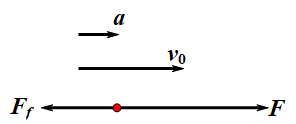
\includegraphics[height=2cm]{4.png}
				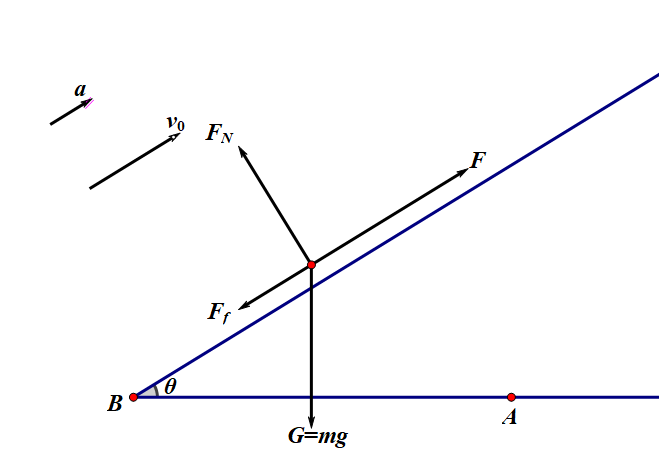
\includegraphics[width=5cm]{5.png}

				\small \textit{Fig. 1 and 2 A cyclist's condition on plain ground and uphill slopes}
			\end{center}

			Since the cyclists will race against each other at a quick speed, the air resistance ($f$) can't be neglected. According to basic physical rules, we can calculate \(f\) with the following formula:
			$$f=\dfrac{1}{2}  C _ D  \cdot \rho_\mathrm{air} \mathrm{S}_\mathrm{body} v^2$$
			where \(C_D\) represents the area facing the wind. To be clear, let
			$$ k _\mathrm{air}=\dfrac{1}{2}  C _ D  \rho_\mathrm{air}$$
			therefore rewriting the previous equation, we have:
			$$f= k _\mathrm{air}\cdot v^2$$
			After searching related data from academic literature, we find out that $ C _ D =0.024$, $\rho_\mathrm{air}=1.293 \mathrm{kg/m}^3$ and $\mathrm{S}_\mathrm{body}=0.209 m^2$. Based on these data, we can indicate that $ k _\mathrm{air}\approx0.0032$.

			According to basic phycial rules (namely \textit{Newton's second law of motion}), we listed the formulae related to motion (\(v\left( t \right) ,a\left( t \right) ,D=s\left( t \right) \)) below (restrictions are also given based on initial set values):
			$$
			\begin{cases}
				\displaystyle
				D=\int^{t_\mathrm{actual}}_0 v(t)\cdot \mathrm{d}t\\
				m \cdot  a (t)=m \cdot v\dot(t)=F-f-mg\sin\left(\theta\right)=\dfrac{P (t)}{v}-\dfrac{1}{2} k_{\mathrm{air}} v^2-mg\sin\left(\theta\right)\\
				v(0)=0\\
				0\leq P (t)\leq m_ b\\
			\end{cases}
			$$

			As for the cyclist, the two variables that will alter his/her performance are mainly \(E(t)\) and \(P(t)\), which respectively indicates the remaining energy and current power at time \(t\).

			Referring to certain articles\cite{114514}, several constants are given below: we define $k$ as the index which describes the restriction of power.
			\[P \dot(t)=-\dfrac{1}{ k } P (t) \cdot \dfrac{1}{ E (t)}\]
			Which means, on a qualitative basis, means that the larger \(P(t)\) is (how hard he/she is riding), and the smaller \(E(t)\) is (how tired he/she is), the faster \(\dot{P(t)}\) will be (he/she will be exhausted more quickly).

			On the other hand, a formula is also needed to relate \(E(t)\) with the previously discussed motional variables. We notice that the derivative of \(E(t)\), or the instant power change, can be described as \(P_{\mathrm{intake}} - P_{\mathrm{output}}\). The second term can be calculated as \(\dot{E}_{\mathrm{output}}=F\cdot \dot{D\left( t \right)} =Fv\left( t \right) \). Therefore, we get the following formulae (restrictions are also given based on initial set values):
			$$
			\begin{cases}
				\displaystyle
				E \dot(t)=\sigma-\left(f+mg\sin\theta+\mu mg\cos \theta\right)\cdot v(t) \\
				E (0)= E _\mathrm{total} \\
				E (t)\geq0,\, \forall\,0 \leq t \leq t_\mathrm{total} \\
			\end{cases}
			$$
			\(\Rightarrow E (t)=\left[\sigma-\left(f+mg\sin \theta +\mu mg \cos \theta \right)\cdot v(t)\right]\cdot t+ E _\mathrm{total}\)

			We substitute the three equation sets above into one equation below:
			\[E (t)=-\dfrac{P (t)}{ k \cdot P \dot(t)}=-\dfrac{mv\ddot(t)+\dfrac{1}{2} k {v(t)}^3}{mv\dot(t)\cdot v(t)+v\dot(t)^2+\dfrac{3}{2} k {v(t)}^2}\]

			To increase reality and accuracy, we notice the fact that not all of the consumed energy can be converted into actual force. Therefore, we add a pre-factor \(\epsilon\) before the \(P_{\mathrm{output}}\). The factor will be calculated through comparations with real-life data. As mentioned before, we use world-record data to achieve this. (Notice that the formulae above also change with the emergece of \(\epsilon\))
			$$ -\dfrac{mv\ddot(t)+\dfrac{1}{2} k {v(t)}^3}{mv\dot(t)\cdot v(t)+v\dot(t)^2+\dfrac{3}{2} k {v(t)}^2} =  \left[\sigma-\epsilon\left(f+mg\sin \theta +\mu mg \cos \theta \right)\cdot v(t)\right]\cdot t+ E _\mathrm{total}$$

			After solving the differential equation above and calculating the appropriate \(\epsilon\), we plot the velocity function \(v\left(t\right)\) as follows:

			\begin{center}
				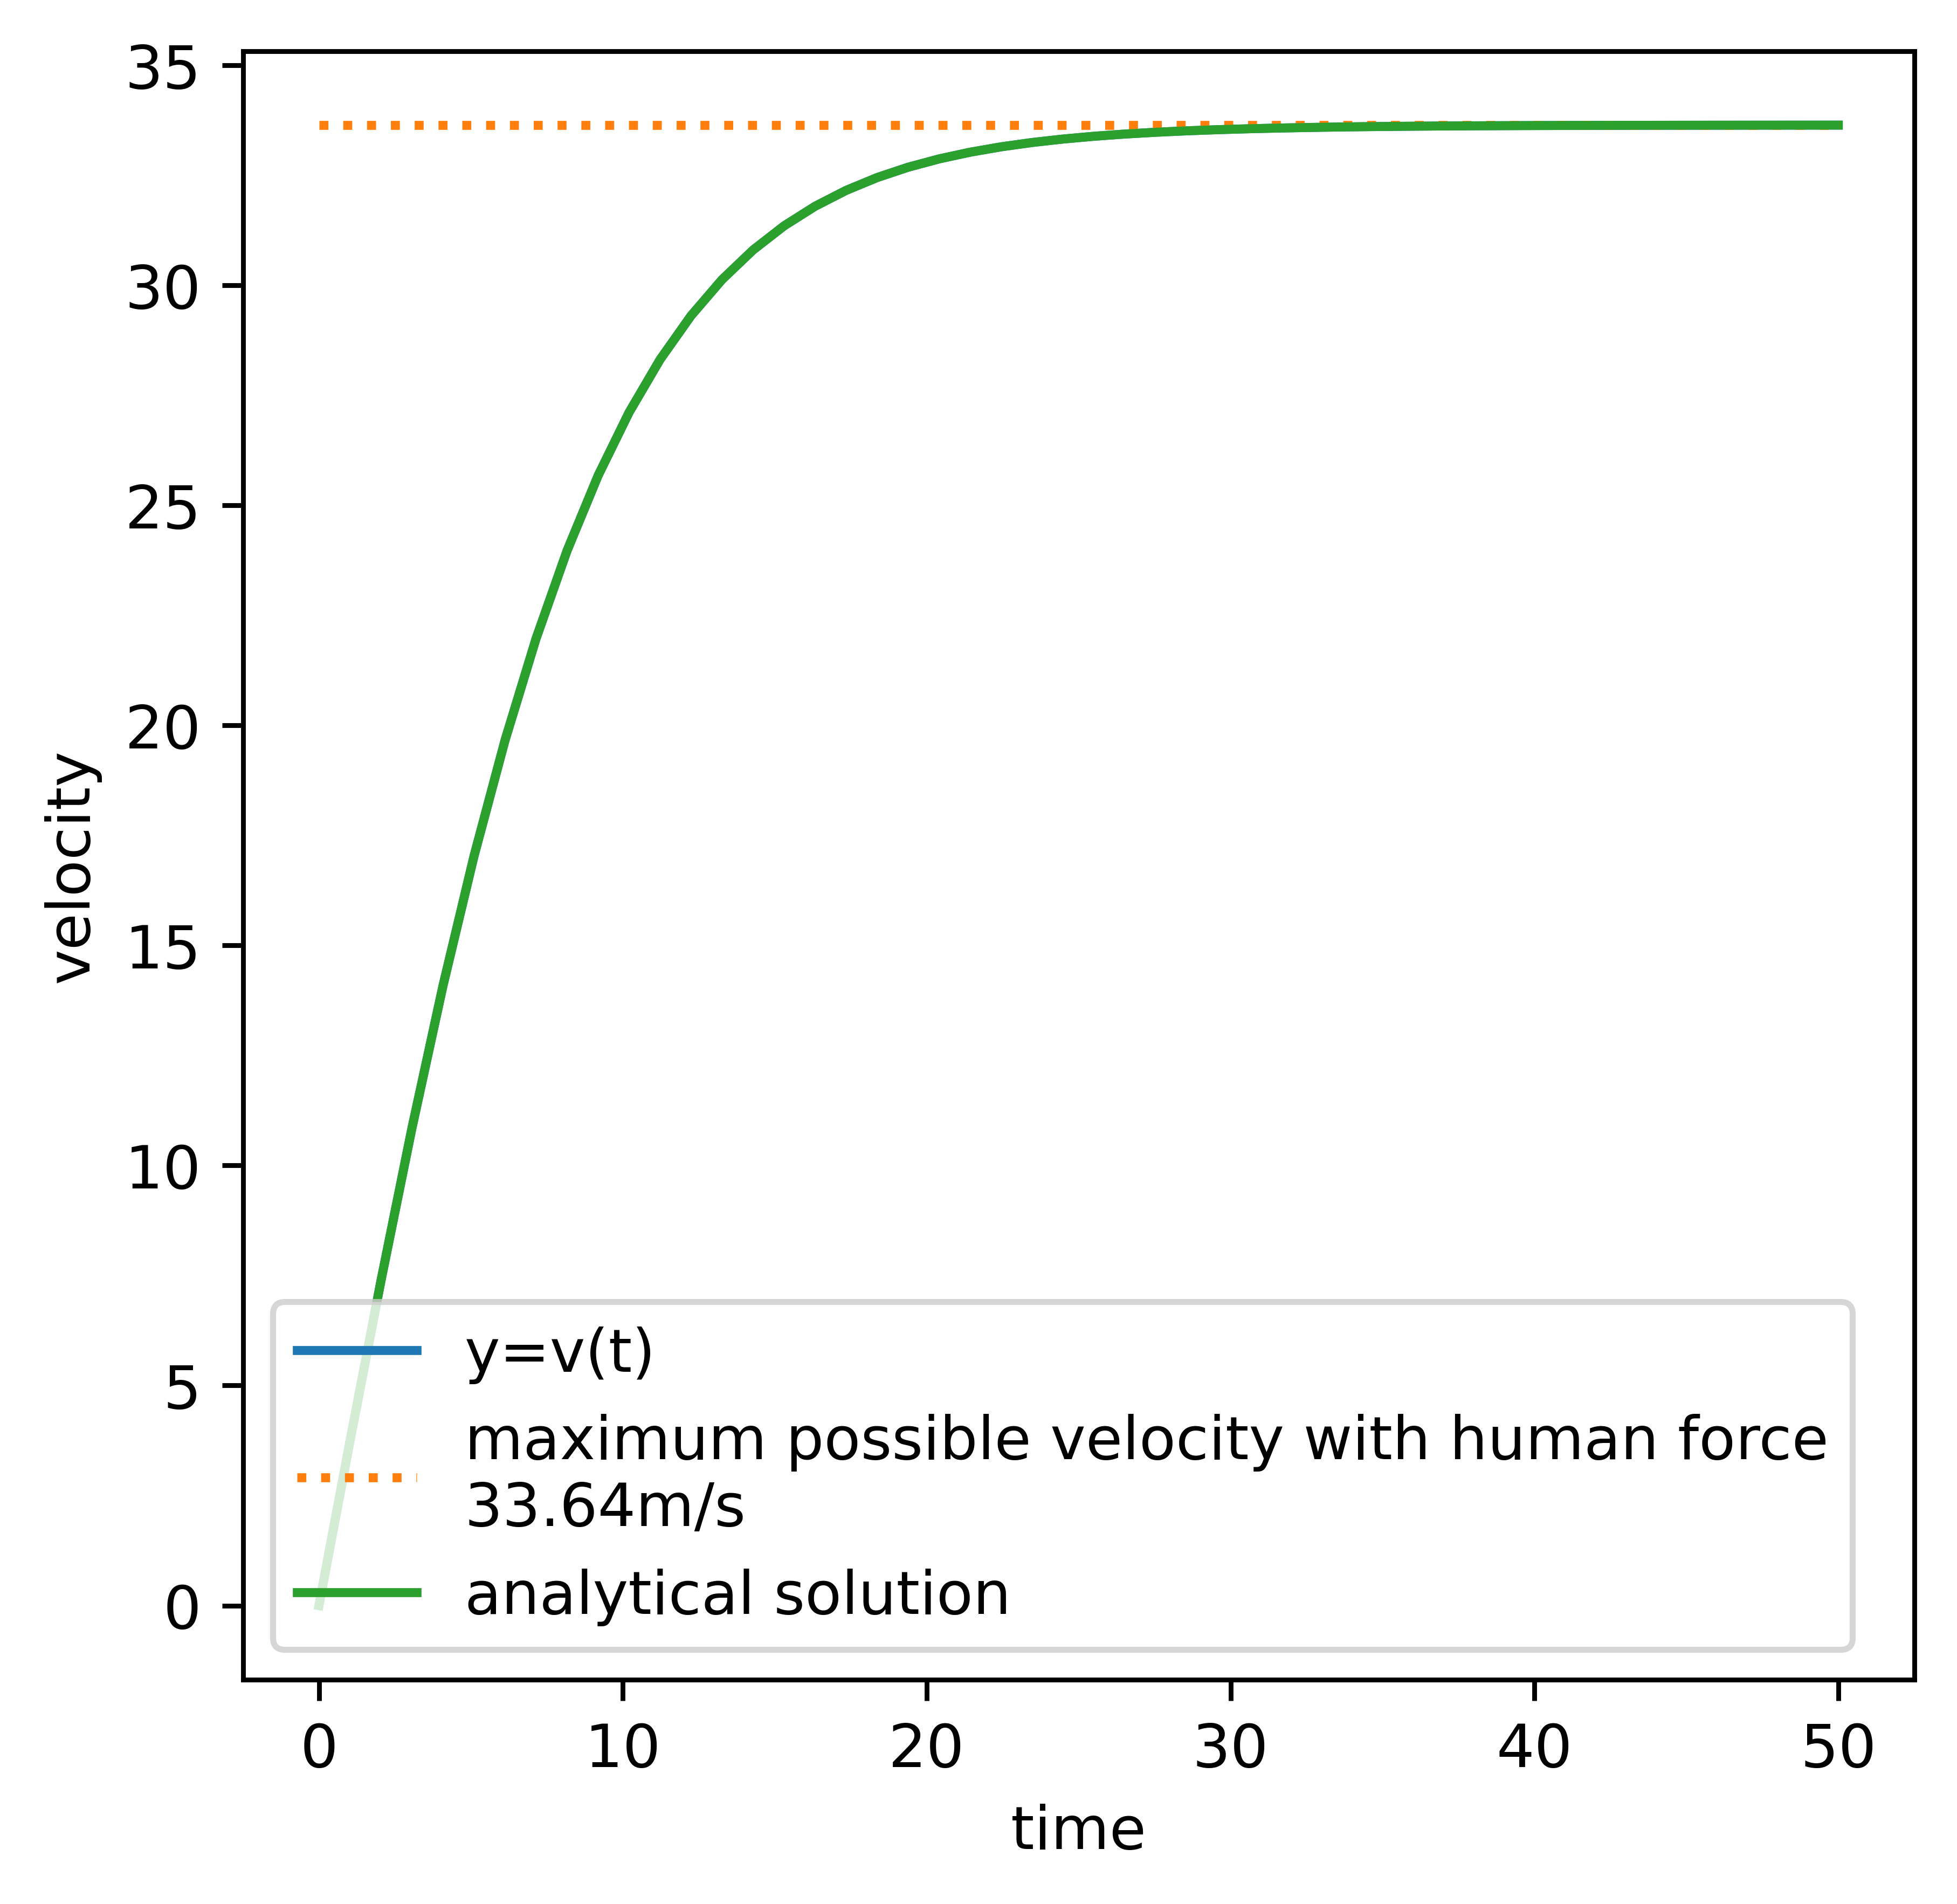
\includegraphics[height=6cm]{1.png}
				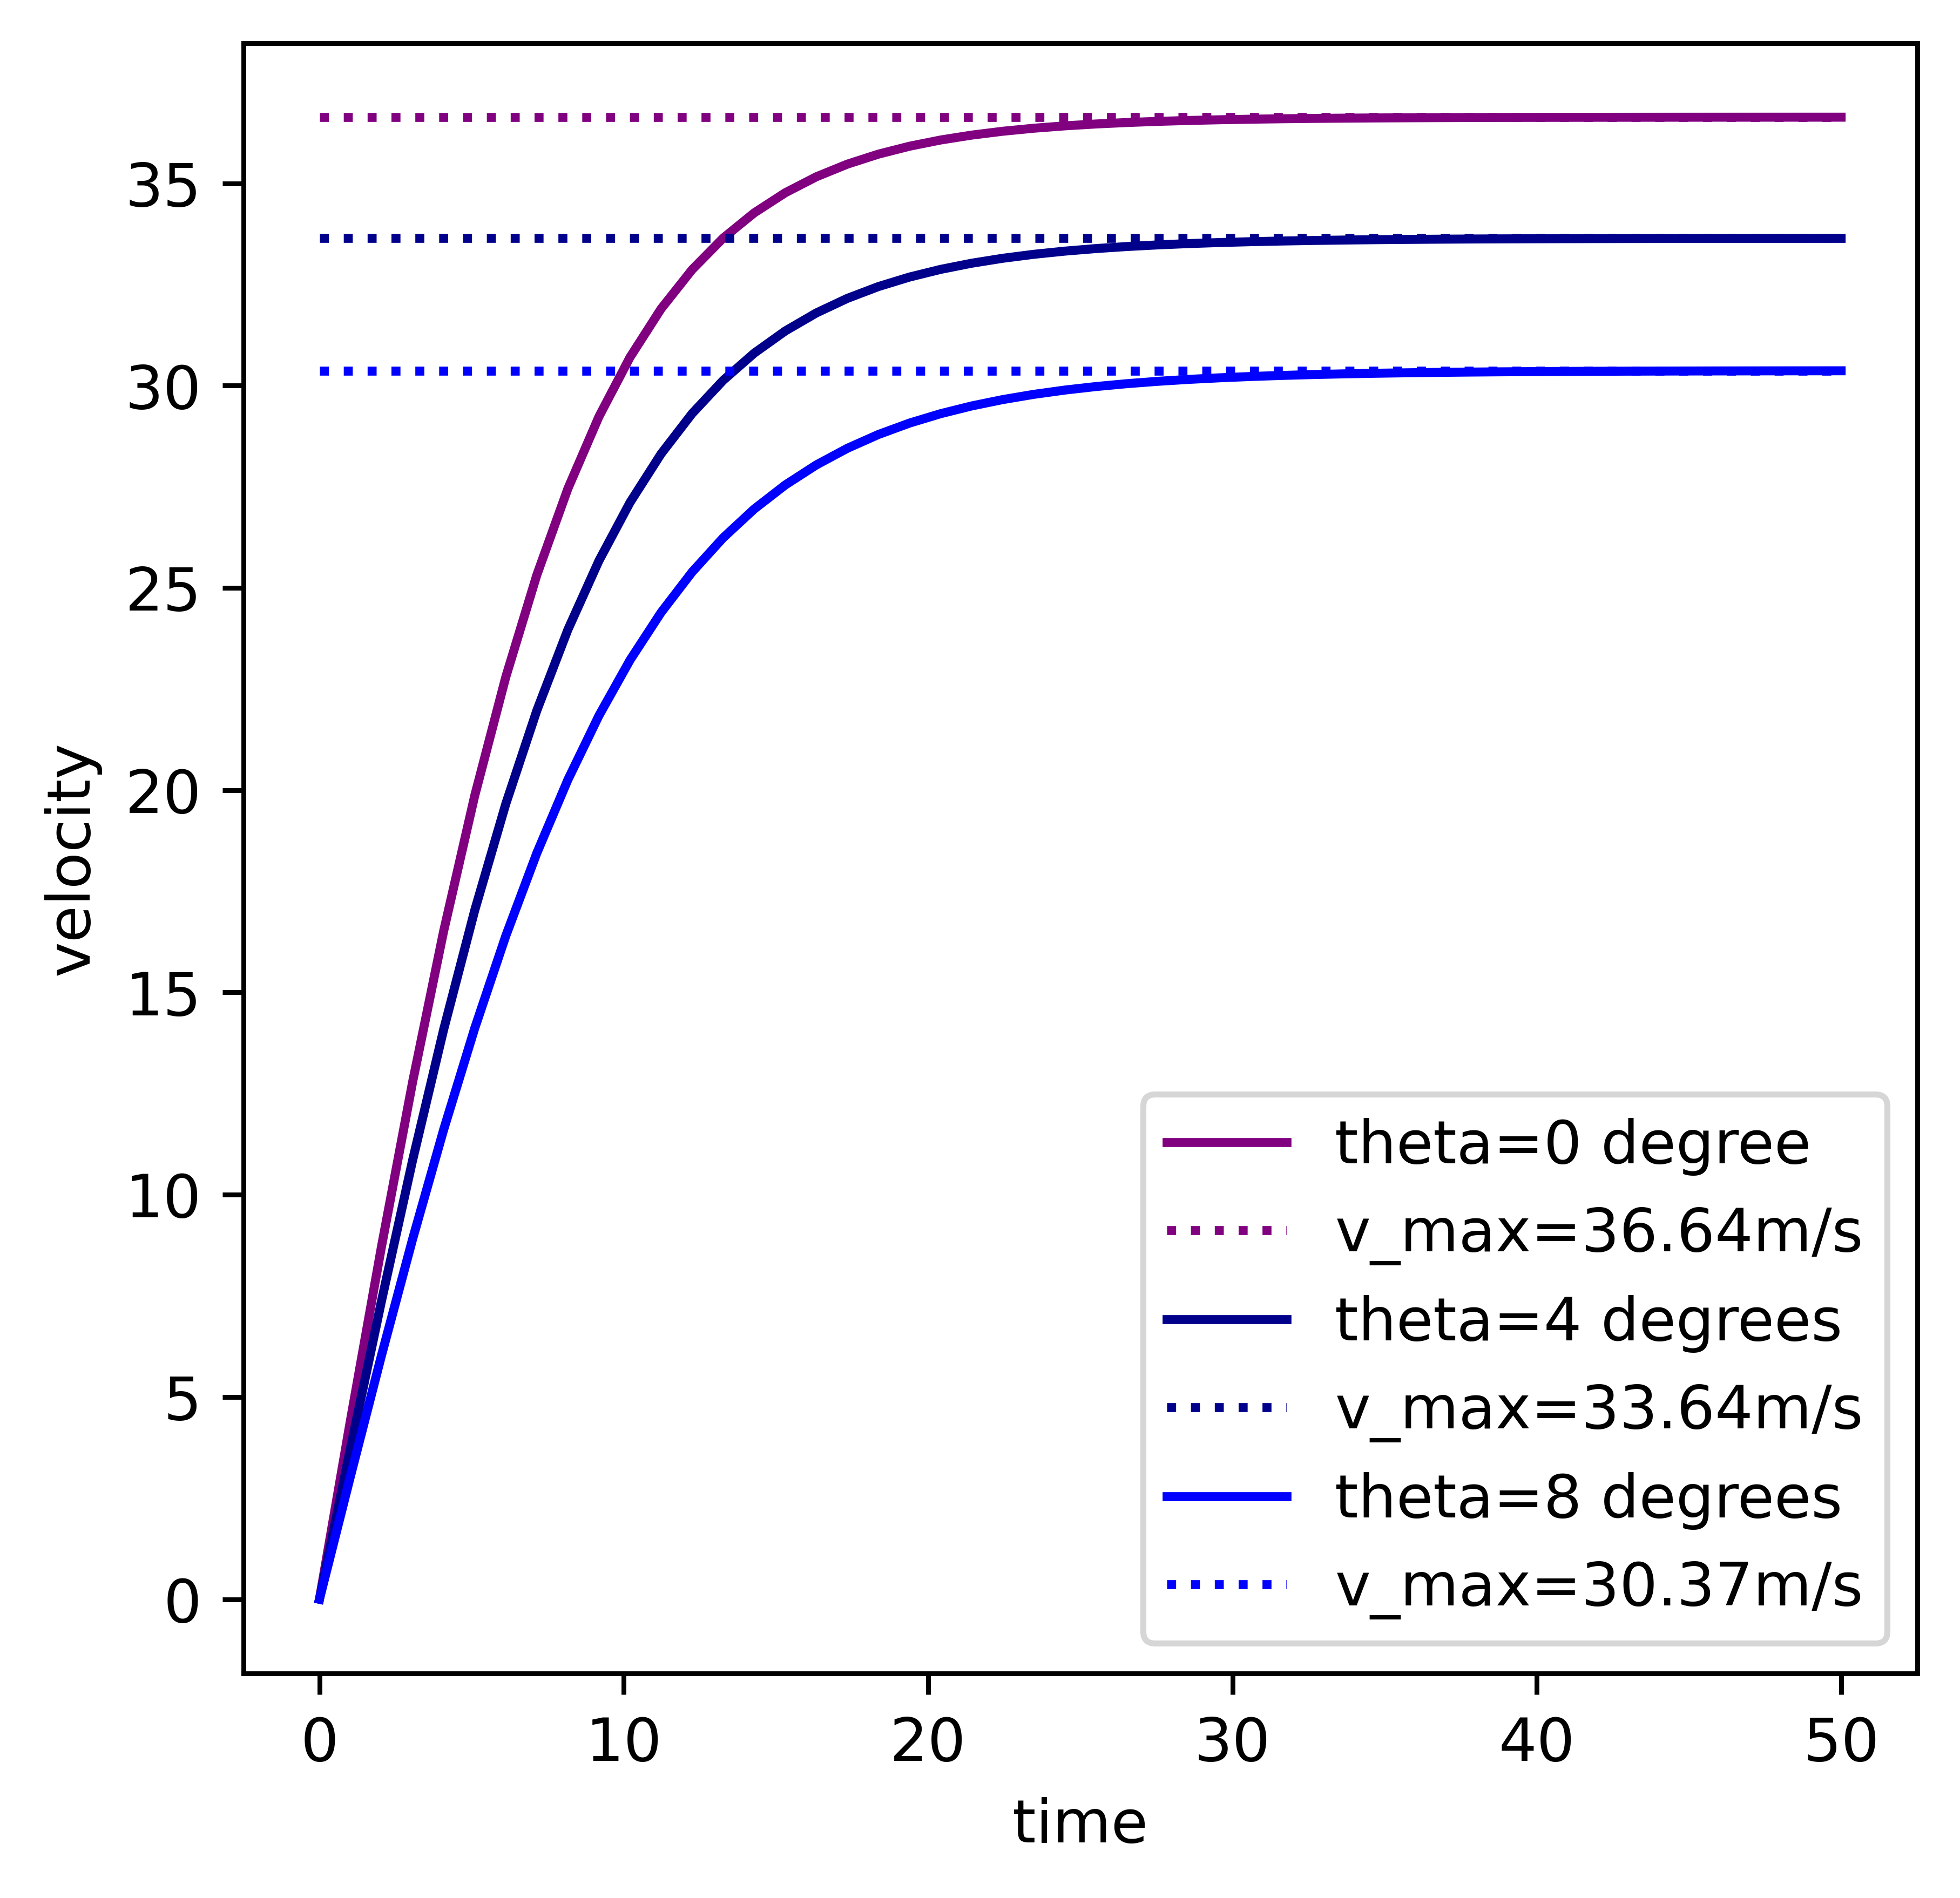
\includegraphics[height=6cm]{2.png}

				\small \textit{Fig. 4 and 5 Patterns of $v(t)$ on different slopes}
			\end{center}

			We also plot function \(E(t)\) as below:
			\begin{center}
				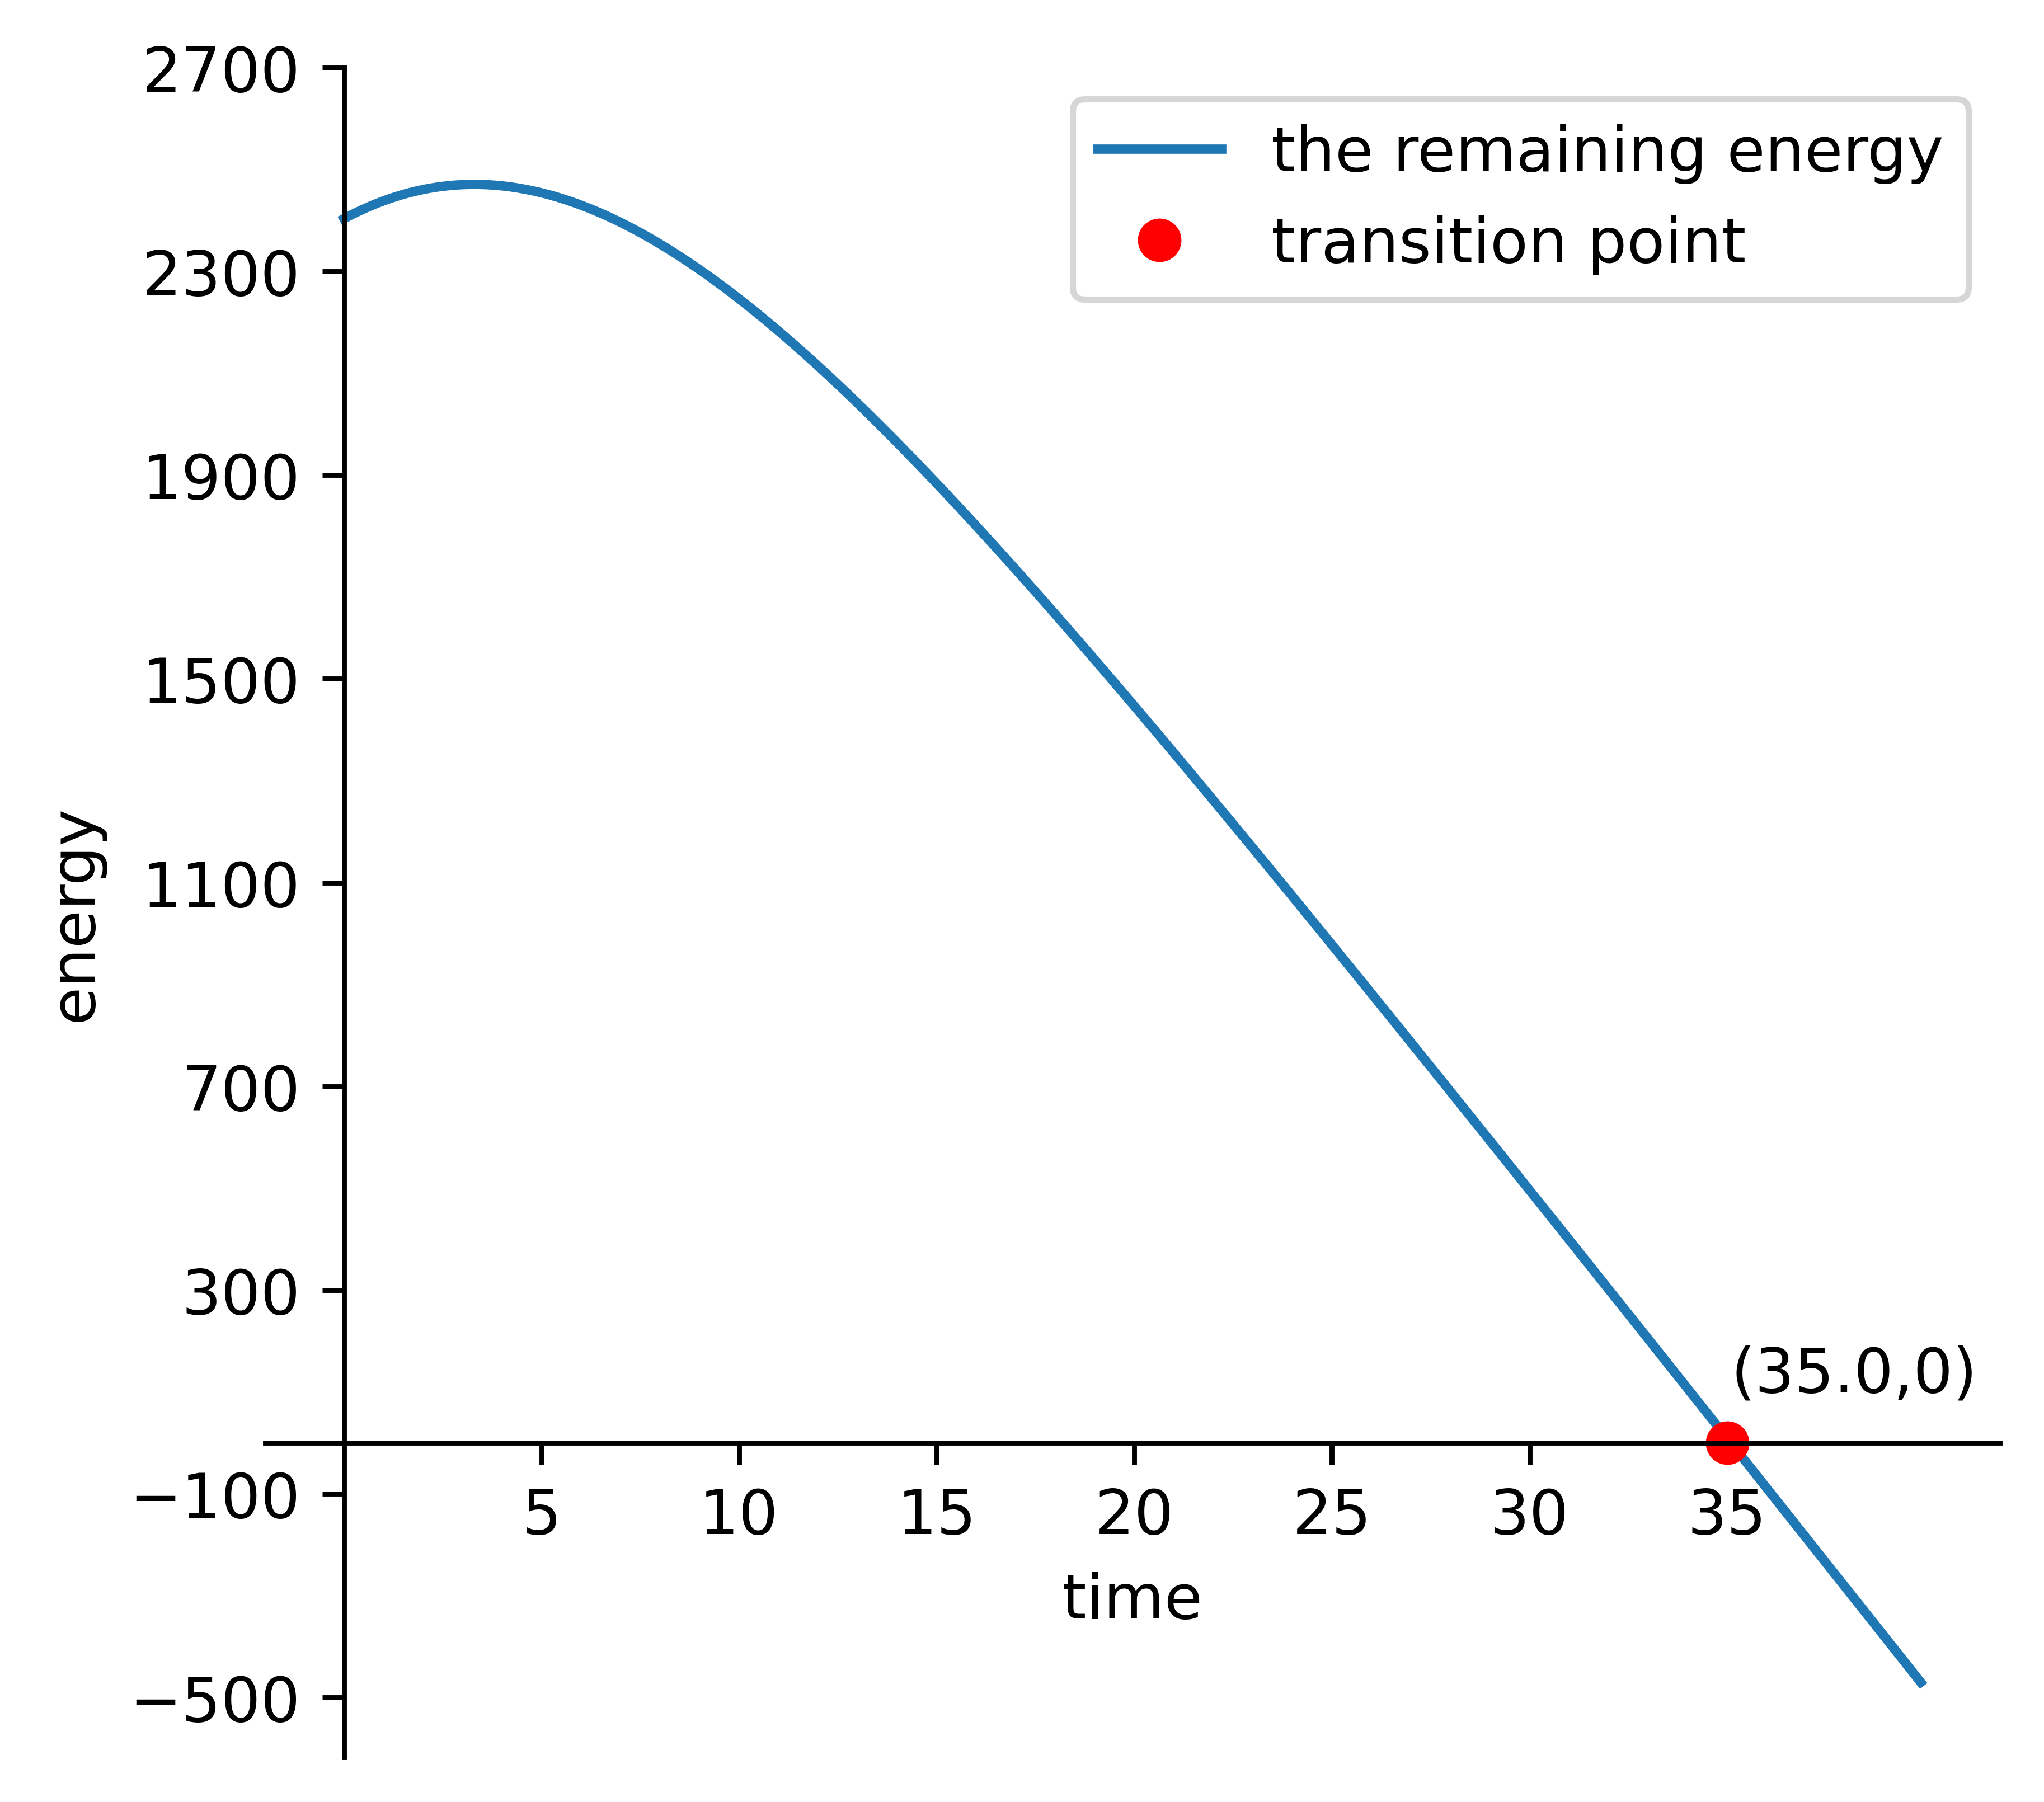
\includegraphics[height=5cm]{3.png}

				\small \textit{Fig. 6 Energy Pattern when dashing}
			\end{center}
			We can find that if a cyclist starts dashing, his/her remaining energy will have a sharp decline. The transition point \(\left(t_0,0\right)\) (the point where \(E(t) = 0\) represents the maximum time a rider can dash at full power before being exhausted. By observing the graph, we can find that \(t_0\) equals 35.0 $\mathrm{s}$. In addition, by integrating the velocity function, we can get the farthest that an athlete can go under this scenario:
			\[D_{\mathrm{first}\:\:\mathrm{phase}}=\int_0^{t_0}{v\left( t \right) \mathrm{d}t}\]
			Finally we find that the maximum dashing distance is 788.3$m$.

		\item For a part that is longer than that $d_{\mathrm{strategy}}\left(\theta\right)$, we choose another strategy: at first, we use a certain amount of energy to \textit{push} the cyclist for a set period of time (which will be discussed later) before it enters the second phase, where the cyclist gradually depletes its energy till it reaches zero. In the end, the cyclist uses his/her remaining inertia to enter the next series (downhill course).
			\begin{center}
				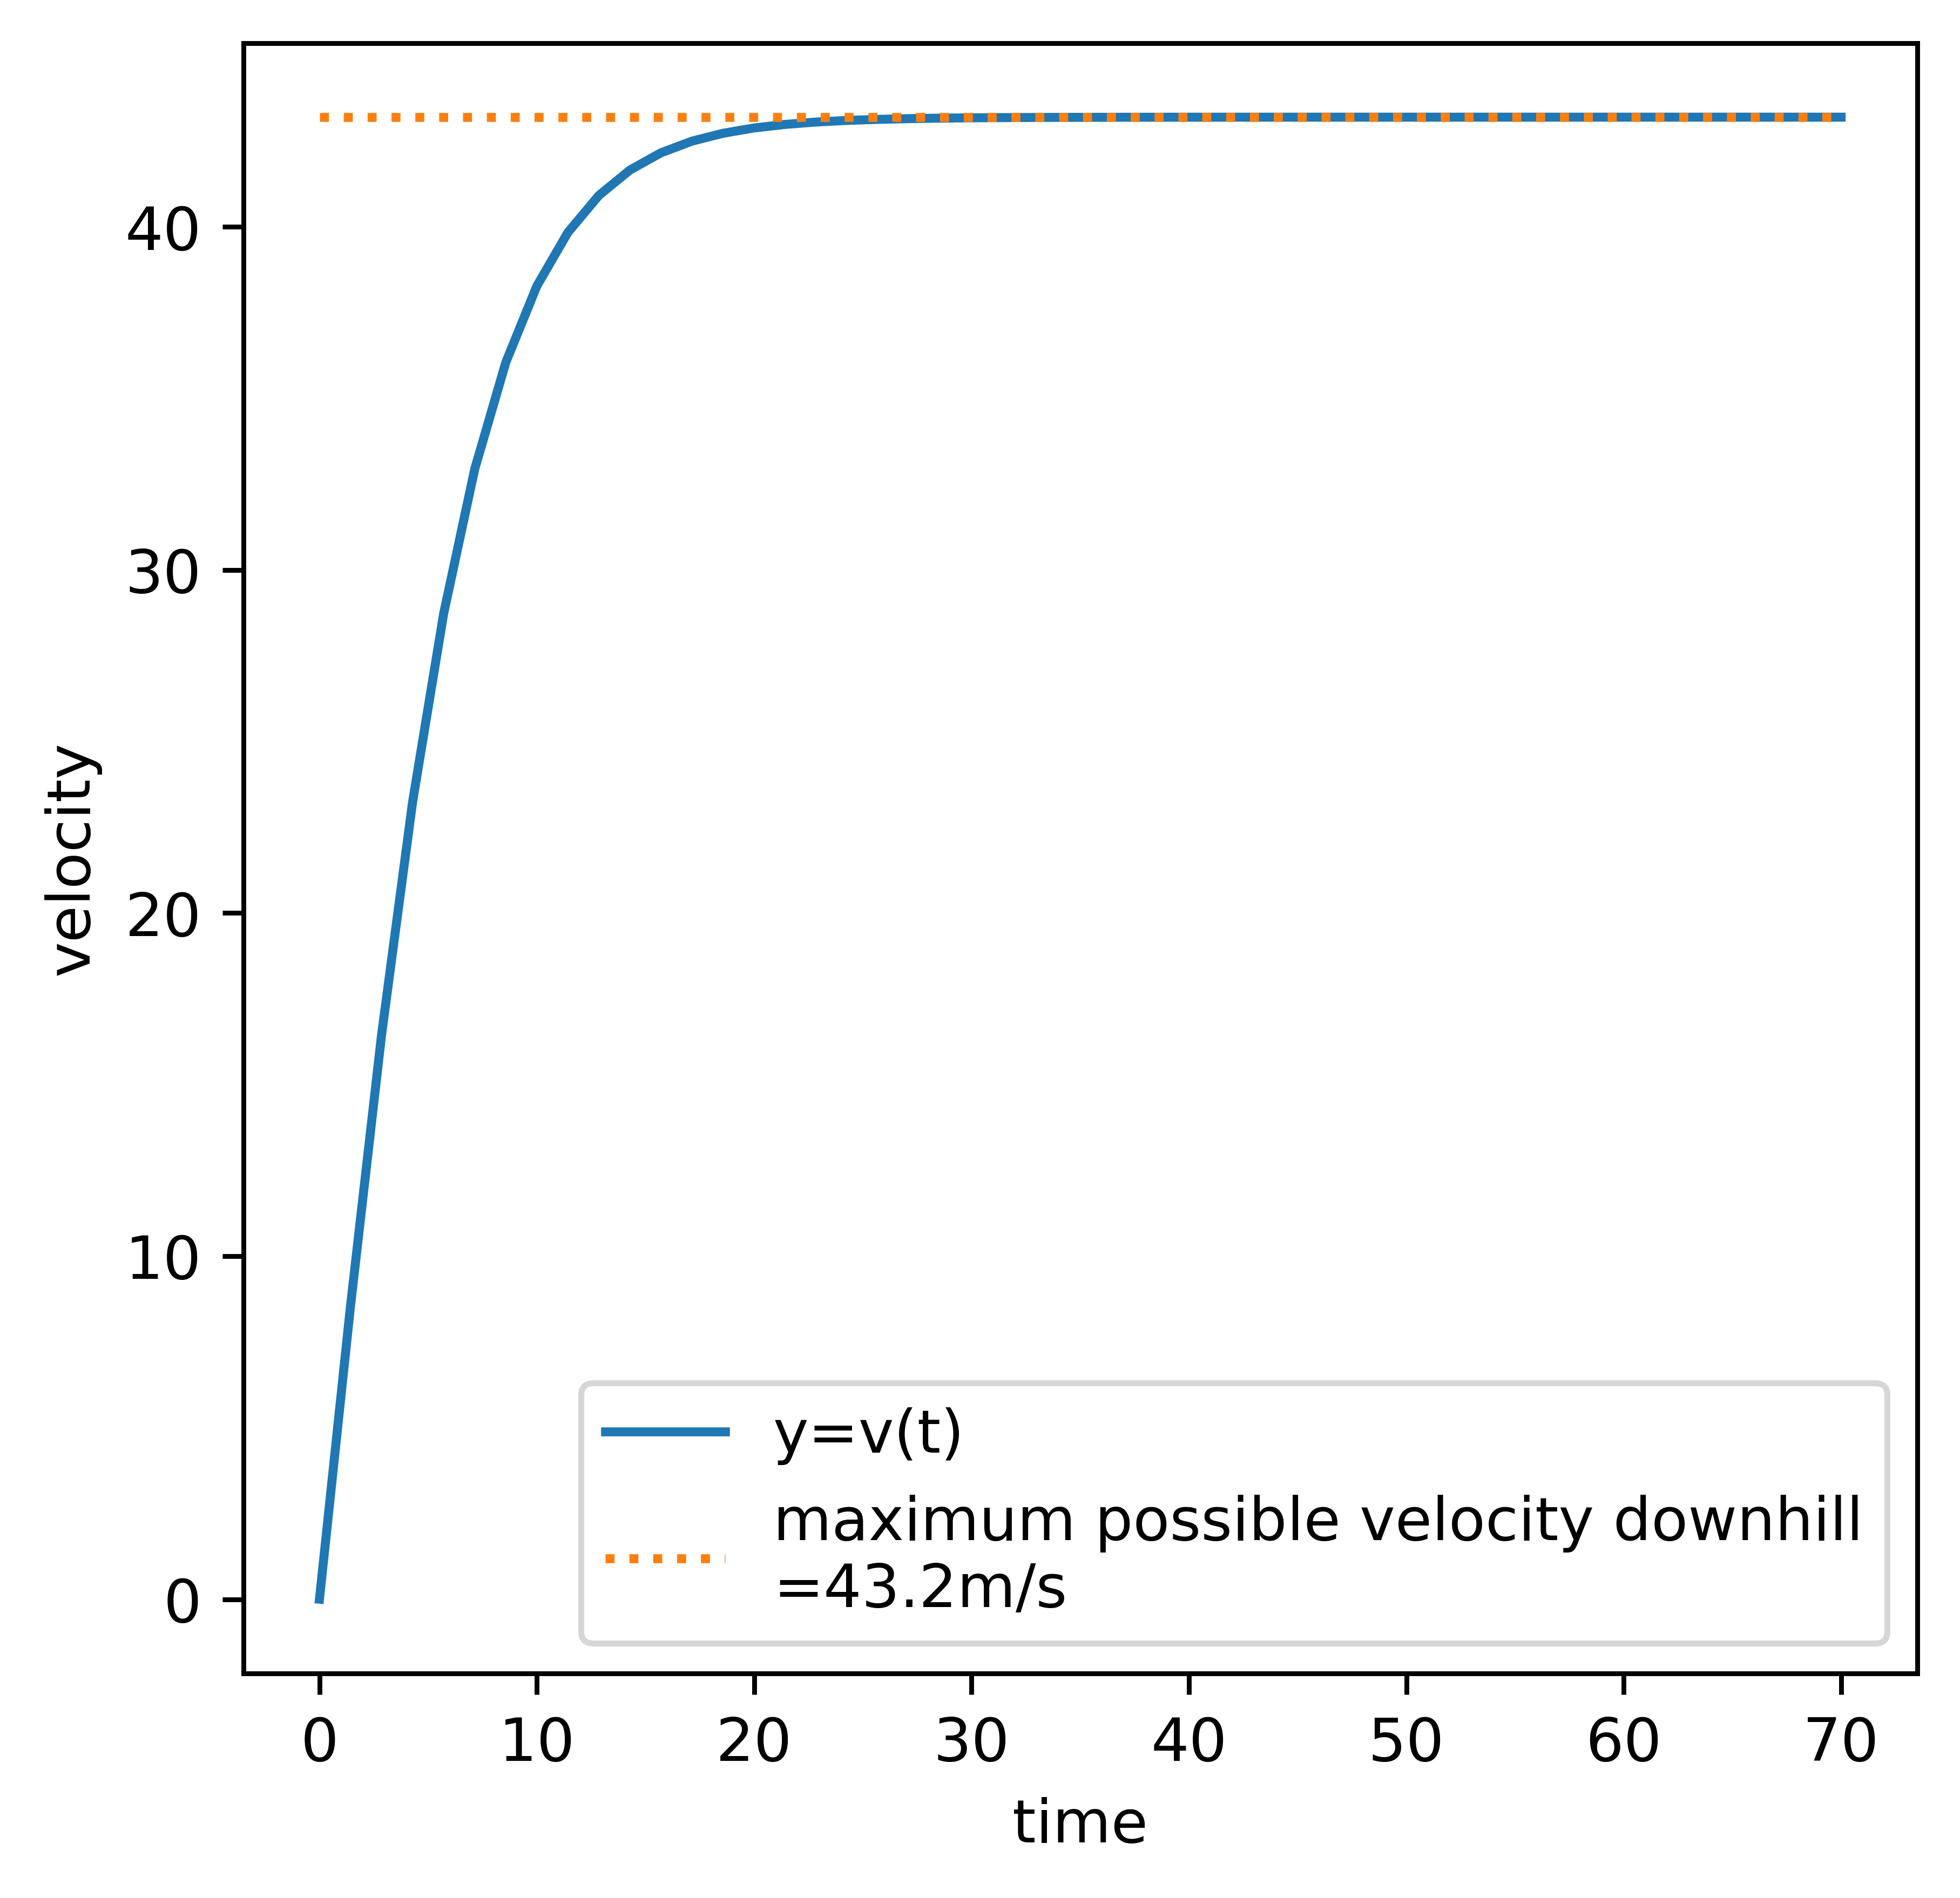
\includegraphics[height = 6cm]{11.png}

				\small \textit{Fig. 7 Velocity pattern while dashing downhill}
			\end{center}

			For the downhill part, we define ($\theta$) as the downhill slope. Therefore, we only need to change the sign before any ($\sin\theta$) term. After altering the formulae, we get the plot above.
	\end{itemize}

	\begin{itemize}
		\item For the downhill part, we define \(\theta\) as the downhill slope. Therefore, we only need to change the sign before any \(\sin\left(\theta\right)\) term. After altering the formulae, we get the plot above.
		\item We divide the rest of the \textit{long} uphill slope (or plane) into three phases (speeding up; maintain a certain speed and dashing at \(E(t)=0\) with inertia).

			Suppose the three phases respectively ends at \(t_1\), \(t_2\), and \(t_{\mathrm{actual}}\). We have the following inter-restrictions on our variables:

			$$
			\begin{cases}
				E \left( t \right) =0,\:\:\forall \:t_2\le t\le t_{\mathrm{actual}}\\
				v_{\mathrm{second}\:\:\mathrm{phase}}\left( t \right) \equiv v_{\mathrm{first}\:\:\mathrm{phase}}\left( t_1 \right)\\
			\end{cases}
			$$
			\begin{enumerate}
				\item \(0\leq t\leq t_1\) (the actual value of \(t_1\) will be discussed later)
					In this phase, the whole process is just like what has been discussed in the \textit{short course} part.
					\[v_1(t)=\dfrac{\sqrt{\mathrm{A}} \tan \mathrm{h}\left[\dfrac{\left(m C _1+t\right)\sqrt{\mathrm{A}k}}{m}\right]}{\sqrt{ k }},\:\:0\leq t\leq t_1\]
					and with this formula, it's easy for us to get the velocity pattern before we turn into the next phase. But first let's see what'll happen during phase 3:
				\item \(t_2\leq t\leq t_{\mathrm{actual}}\) (the actual value of \(t_2\) will be discussed later)
					We use the restriction \(E_{\mathrm{third\:\:phase}}\equiv 0\), and therefore:
					\[0=E \dot(t)=\sigma-\left(f+mg\sin\theta+\dfrac{mgu}{r_{\mathrm{wheel}}}\right)\cdot v_3(t)\]
					Substitute the derivative of \(v_3(t)\) into :

					\(m \cdot v\dot(t)=\underset{\mathrm{which\:\:equals\:\:}0}{\underbrace{\dfrac{P (t)}{v}}}-\dfrac{1}{2} k_{\mathrm{air}} v^2-mg\sin\left(\theta\right)\) 

					We solve that:

				\item \(t_1\leq t\leq t_2\)
					We calculate the whole distance of the process using integral:
					\[D(v(t))=\int_0^{t_1}v_1(t)dt+v_2(t_2-t_1)+\int_{v_2}^{t_{\mathrm{actual}}}v_3(t)dt\]

			\end{enumerate}
	\end{itemize}

	\subsubsection{Splicing}
			Now that we've successfully developed a set of strategies that can be applied to a single slope or plain. To get the whole picture of $v(t)$, we need to divide the whole course into several \textbf{series} as mentioned above. Therefore, a clear definition of a \textbf{turning point} is needed.

			After this, for a specic course plot, we connect all the adjacent \textbf{turning points} and apply our strategies to each of the connected segments, only with these two variables changed:
			$$
			\left\{ \begin{array}{c}
				v\prime\left( 0 \right) =v_{\mathrm{end}\:\:\mathrm{of}\:\:\mathrm{last}\:\:\mathrm{section}}\\
				E\prime\left( 0 \right) =E_{\mathrm{end}\:\:\mathrm{of}\:\:\mathrm{last}\:\:\mathrm{section}}\\
			\end{array} \right.
			$$
			However, it's also important to note that the \textit{splicing} only works well with relatively regular (especially, \textbf{linear}) changes in the slopes. Those with irregular courses will be discussed in the next model.

	
	\section{Model B}
	\subsection{Model Overview}
	In this model, we will firstly discuss how to descibe rider's basic feature and their power curve in detail. Later, we will also take special factors such as climate ino consideration. Finally, we will apply our model into several world-famous time trial courses to justify our deductions. As mentioned above, model B is applicable to all patterns of slopes, making it more universal but also more complicated than model A.
	\begin{enumerate}
		\item	\textbf{Rain is not considered in this model.}

				Many activities have been cancelled or delayed because of rainy days in the past few years. But if the trial's humidity is under the criteria. Roads' dynamic coefficient of friction won't be affected.
		\item \textbf{The change in air density and air pressure can be neglected}

				Unlike mountain bike races, the change in altitude is small enough (\(\leq 200\mathrm{m}\)) to be neglected in the atmospherical scope.
	\end{enumerate}
	\subsection{Notation}
	\begin{tabular}{|l|l|l|}
		\hline
		$m(\mathrm{x})$&weight of cyclist&$\mathrm{kg}$\\
		\hline
		$\mathrm{h}(\mathrm{x})$&height of cyclist&$\mathrm{m}$\\
		\hline
		$\mathrm{BMI}(\mathrm{x})$&body mass index of cyclist&/\\
		\hline
		$E_\mathrm{total} (\mathrm{x})$&total energy of cyclist&$\mathrm{J}$\\
		\hline
		$\mathrm{S}_\mathrm{body}(\mathrm{x})$&body measure&$\mathrm{m}^2$\\
		\hline
		$t_\mathrm{min}$&the least time spent to complete the game&$\mathrm{s}$\\
		\hline
		$F_\mathrm{wind}$&wind force&$\mathrm{N}$\\
		\hline
		$T$&temperature of the trial&$^{\circ}\mathrm{c}$\\
		\hline
		$\mathrm{K}_b$&the Boltzmann constant&/\\
		\hline
		$\epsilon$&attenuation factor&/\\
		\hline
	\end{tabular}
	\subsection{Calculate Total Energy}
	In this part, we will mainly discuss the cyclist's total power based on his phisycal condition and cycling type. 

	First, we need to have a basic understanding of the cyclist's physical condition. Take Tour de France as an example\cite{france}. Among the champions of this race in the past five years, their average height is 1.808$\mathrm{m}$ and their average weight is 68.58$\mathrm{kg}$. Olympic cyclists have an average height of 1.80$\mathrm{m}$ and an average of around 68$\mathrm{kg}$\cite{weight}. 

	Next, we quantify the attributes of a cyclist with two indicator variables: \(L\) represents the cyclist's adaptability to new terrains, or the \textbf{learning rate}, which will later be introduced in the algorithms. The higher \(L\) is, the more quickly the rider will change his/her strategy during the course. Another indicator \(\epsilon\), which has already been mentioned before, measures the rider's capability of converting force into dynamics.

	To achieve this, we used the neural networks algorithm to get these two indicators by fitting them into previous records. Relative calculations have already done in the physical analysis part in model A. The process is shown below:

	\begin{center}
		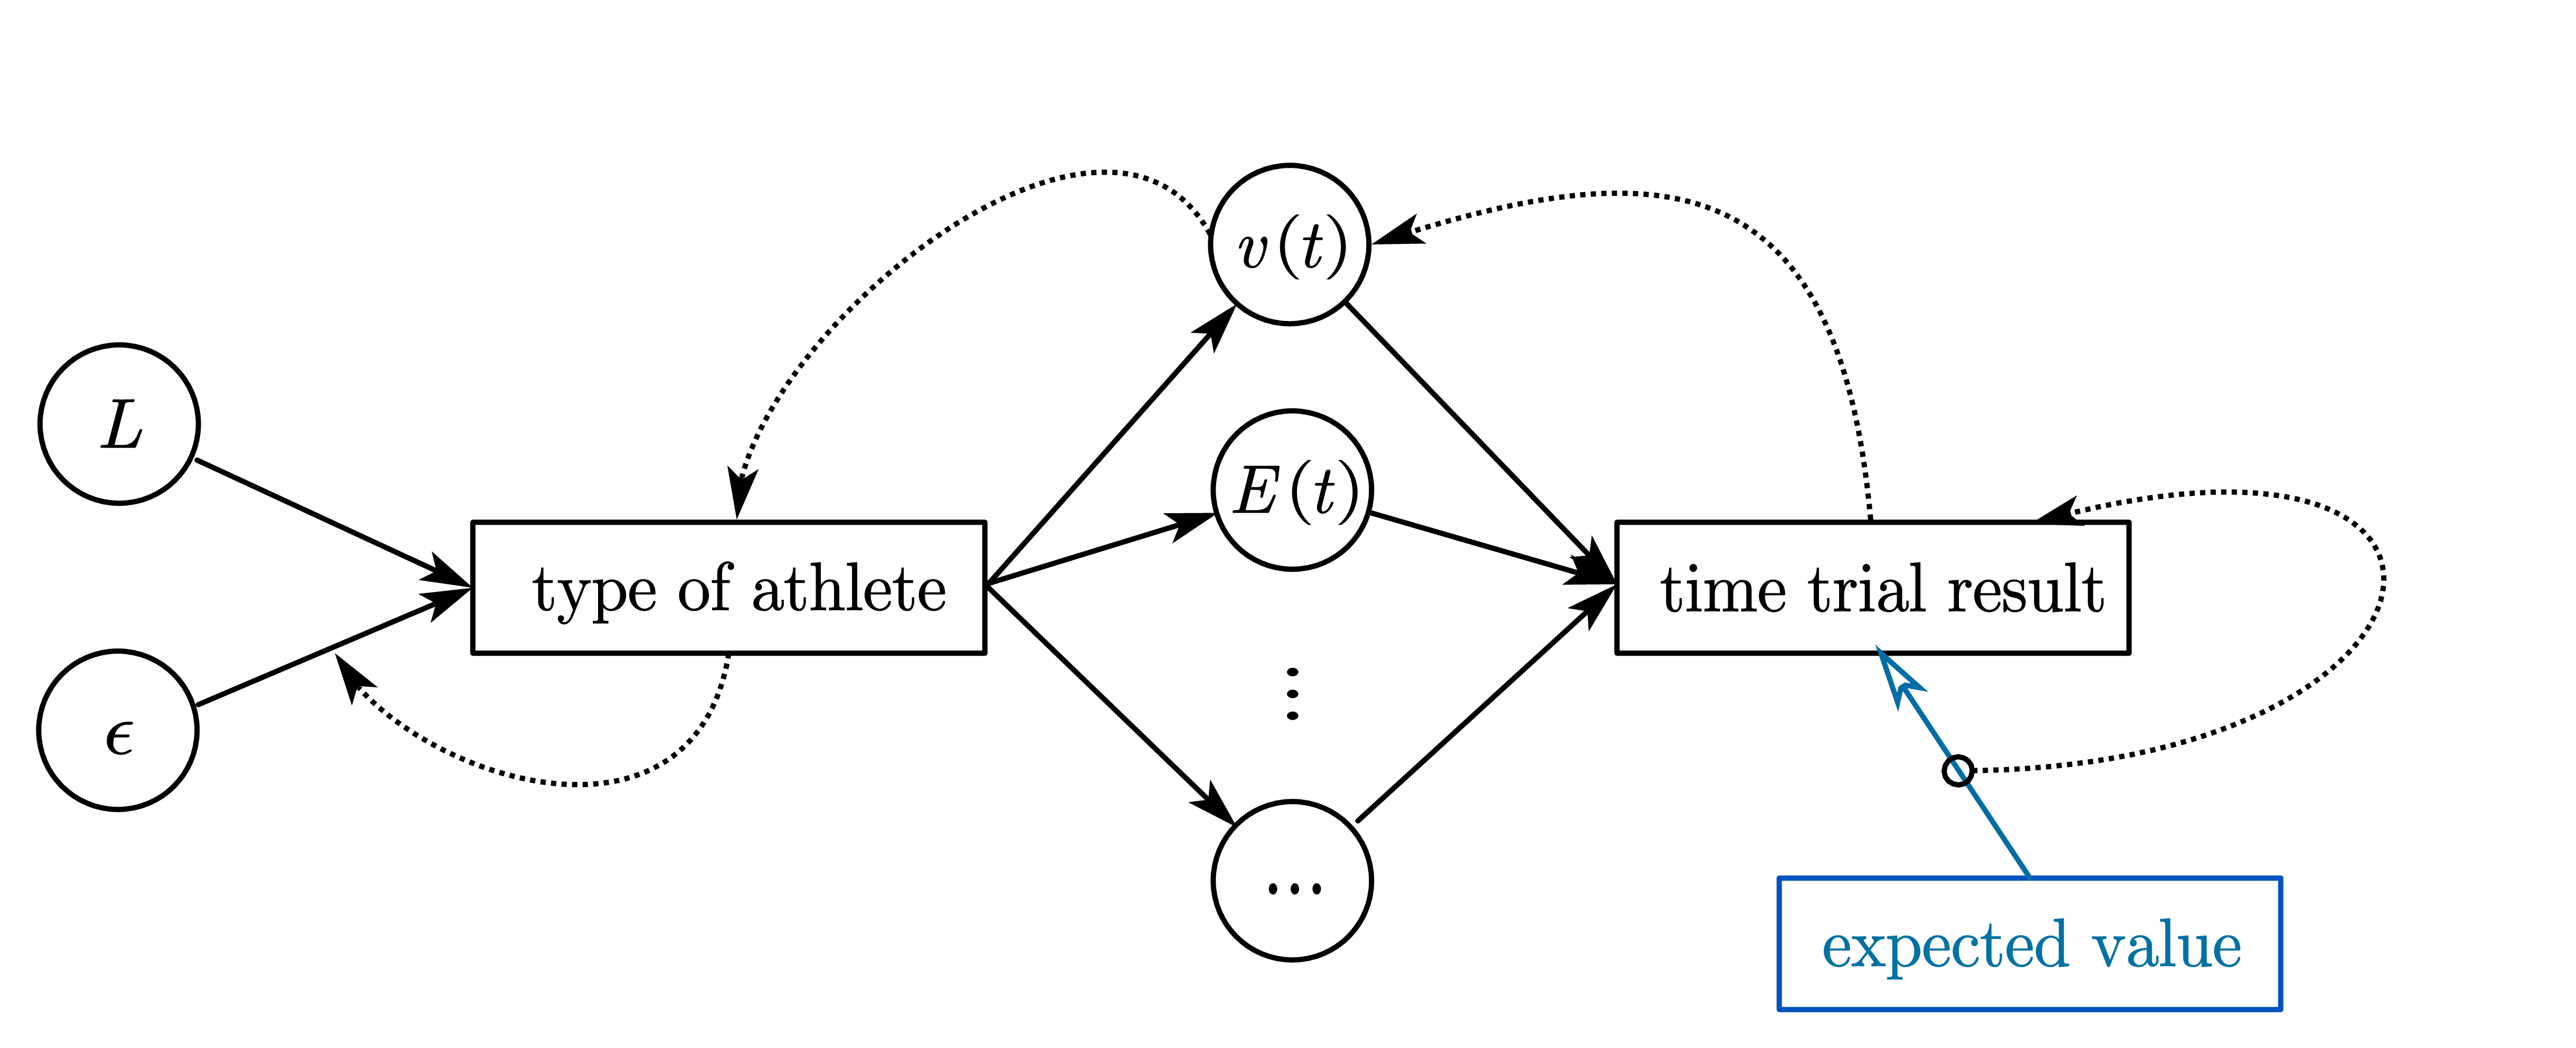
\includegraphics[height = 6cm]{10.png}

		\small\textit{Fig. The working process of the neural network}
	\end{center}

	Then we randomly pick the parameters and put it into practice using the formulae:

	\[
		\boxed{\mathrm{randomly\:\:put\:\:weights\:\:on\:\:two\:\:edges}} \\
		\leftarrow
		\boxed{\mathrm{randomly\:\:choose\:\:parameters\:}L\mathrm{\:and\:}\epsilon} \
		\]

	\(
		\downarrow
		\)

	\[
		\boxed{\mathrm{calculate\:\:the\:\:relavent\:\:variables\:(E.g\:}v(t))} \rightarrow
		\boxed{{\mathrm{get\:\:the\:\:final\:\:result\:\:of\:\:time\:\:trial}}}
		\]

	We compare the standard difference \(\left( r_{\exp}-r_{\mathrm{act}} \right) ^2\) between the expected value and the actual calculated one, and make renders to the parameters. In the end, we got the results when the parameters became relatively stable, as shown below:

			\begin{center}
				\begin{tabular}{|l||c|c|c|c|c|}
					\hline
					&\textbf{time trial specialist} & \textbf{climber} & \textbf{rouleur} & \textbf{sprinter} & \textbf{puncheur} \\
					\hline
					\hline
					\(L\) & 0.95 & 0.74 & 0.90 & 0.65 & 0.82 \\
					\hline
					\(\epsilon\) & 0.85 & 0.91 & 0.90 & 0.70 & 1.00 \\
					\hline
				\end{tabular}
			\end{center}

			In our model, we use a series of variables with (\(x\)) to describe the cyclist's features. These include $m( x )$, $ h ( x )$, etc. According to the BMI criteria, we can get the formula:
			$$\mathrm{BMI}( x )=\dfrac{m( x )}{ h ^2( x )}$$
			Also, since where our body is exposed to air can be seen as a rectangle, we can approximately get that:
			\[S_{\mathrm{body}} \propto \mathrm{BMI}(x)\cdot h(x)\]
			\[\Rightarrow S_{\mathrm{body}}=k\cdot \dfrac{m(x)}{h(x)}\]
			The total energy can also be given by a weighted sum of the parameters listed:
			\[E_{\mathrm{total}}=-k_1\cdot\mathrm{Gender}(x)+k_2[m(x)-w_0]^2+k_3\cdot A\cdot [\mathrm{Age}(x)]+k_4\]
			where
			\[A(x)=
				\begin{cases}
					k_5\left\{\sin\left[\dfrac{(x-15.5)\pi}{31 }\right]+1\right\}~~~,~x\leq 31 \\
					-k_6 (x-31)^2+2k_5~~~~~~~~~~~~~~,x>31
				\end{cases}
			\]
			and according to \cite{114514}, \(\max\{E_{\mathrm{total}}\}\approx 2403.5 \mathrm{J} E_{0}\). By searching the internet \cite{energy curve}, we can find that a pesron reaches his/her maximum energy at the age of 31.
			\[
				\Rightarrow
				\begin{cases}
					\lim\limits_{x\rightarrow 31^+} A\left( x \right) =\lim\limits_{x\rightarrow 31^-} A\left( x \right)=E_0 \\
					A(60)=\dfrac 12 E_0
				\end{cases}
			\]
			Therefore, \(k_5 = \dfrac{E_0}{2}\) and \(k_6=\dfrac{k_5}{841}\).
	\subsection{Weather Conditions}
	Weather condition also plays a vital part in the cyclists's strategy. In this part, we will mainly discuss two kinds of weather condition: temperature and wind force.
	\subsubsection{Temperature}
	Temperature mainly has an impact on human's speed of metabolism. 20$^{\circ}\mathrm{c}$ to 30$^{\circ}\mathrm{c}$ is the zone where human can complete physical actions in the most comfortable way. If the environment's temperature is over or below this number, speed of metabolsim will decline. The greater the difference is ,the more quickly the speed decline. Therefore we can get the following formula:
	$$ \sigma\propto e^{-\frac{ E _\mathrm{total}}{\mathrm{K}_ b t}}$$
	($\mathrm{K}_ b $ here refers to the Boltz constant which equals $1.38\times10^-16$ per degree calcius)
	\subsubsection{Wind Force}
	Secondly, we need to discuss the wind force. Since there is wind disturbing the cyclists, we can assume that air resistance no longer exists. This picture below shows the situation where a rider is facing the wind. So we can get the following formula:
	$$\mathrm{F}_\mathrm{wind}=\rho_\mathrm{air}\cdot\mathrm{S}_\mathrm{body}\mathrm{v}^2$$
	Now we can analyze the cyclist's overal stress distribution, which is:
	$$F_\mathrm{total}=-\frac{1}{2}C_\mathrm{D}\rho sv^2+C_\mathrm{D}\rho sv_{wind}v-(mgsin\theta+\frac{1}{2}C_\mathrm{D}\rho sv_{wind}^2+\frac{mg\mu}{r})$$
	\subsection{Recalculate Speed Function}
	After we have discussed the weather's impact on our model, we need to polish it so that it can be applied to special cases as well. Considering that there is no air resistance but wind force now, we need to recalculate the speed function.
	$$\mathrm{v}\dot(\mathrm{t})=\dfrac{-\dfrac{\mathrm{m}\mathrm{v}\dot(\mathrm{t})\mathrm{v}(\mathrm{t})+\dfrac{1}{2}\mathrm{k}{\mathrm{v}(\mathrm{t})}^3}{\left[\sigma-\left(f+mg \sin \theta+\mu mg \cos \theta\right)\cdot\mathrm{v}(\mathrm{t})\right]\mathrm{t}+\mathrm{E}_\mathrm{total}}-\left(\mathrm{v}(\mathrm{t})^2+\dfrac{3}{2}\mathrm{k}\mathrm{v}(\mathrm{t})^2\right)}{\mathrm{m}\cdot\mathrm{v}(\mathrm{t})}$$
	If the momentum is a constant number (which we define as $F(t)$), we can get the following formulae:
	$$mv\dot(t)=F(t)-f-F_{f}-mg\sin \theta=F(t)- k _\mathrm{air}{v(t)}^2-\dfrac{mg\mu}{\mathrm{r}_\mathrm{wheel}}-mg\sin \theta$$
	$$v(0)=0$$
	$$0\leq F(t)\leq F_{m}$$
	and:
	$$ E \dot(t)=\sigma-F(t)\cdot v(t)$$
	$$ E (0)= E _\mathrm{total}$$
	$$ E (t)\geq0$$
	To facilitate our calculation, we define $A$. The definition fromula is as follow:
	$$\mathrm{A}=F_m-\dfrac{mg\mu}{\mathrm{r}_\mathrm{wheel}}-mg\sin \theta$$
	Finally, we combine all the factors together and get the formulae:

	\begin{footnotesize}
		$v(t)\\=\dfrac{\sqrt{F_m-\dfrac{mg\mu}{\mathrm{r}_\mathrm{wheel}}-mg\sin \theta} \tan \mathrm{h} \left(\dfrac{\sqrt{F_m-\dfrac{mg\mu}{\mathrm{r}_\mathrm{wheel}}-mg\sin \theta}\ \ \mathrm{C}\sqrt{ k _\mathrm{air}} m+\sqrt{F_m-\dfrac{mg\mu}{\mathrm{r}_\mathrm{wheel}}-mg\sin \theta}\ \ \sqrt{ k _\mathrm{air}} x}{m}\right)}{\sqrt{ k _\mathrm{air}}}$

		$=\dfrac{\sqrt{\mathrm{A}} \tan \mathrm{h}\left[\dfrac{\left(m\mathrm{C}_1+\mathrm{x}\right)\sqrt{\mathrm{Ak}}}{m}\right]}{\sqrt{ k }}$
	\end{footnotesize}

	$v(0)=\dfrac{\sqrt{\mathrm{A}} \tan h \left(\mathrm{C}_1\sqrt{\mathrm{Ak}}\right)}{\sqrt{ k }}$

	By doing this we can get the result: $\mathrm{C}_1=0$
	\subsection{Applying to Reallife Trials}
	Now that we have figured out the power pattern of cyclists, we can apply it to trials and find out whether it is sensitive in real life. There are three trial courses in our model. The first is 2021 Olympic Time Trial course in Tokyo, the second is 2021 UCI World Championship time trial course in Flanders. Both of the courses has the same features: they have at least one sharp turn and numerous gentle slopes.

	\begin{center}
		
\includegraphics[width=15cm]{6.png}\\
		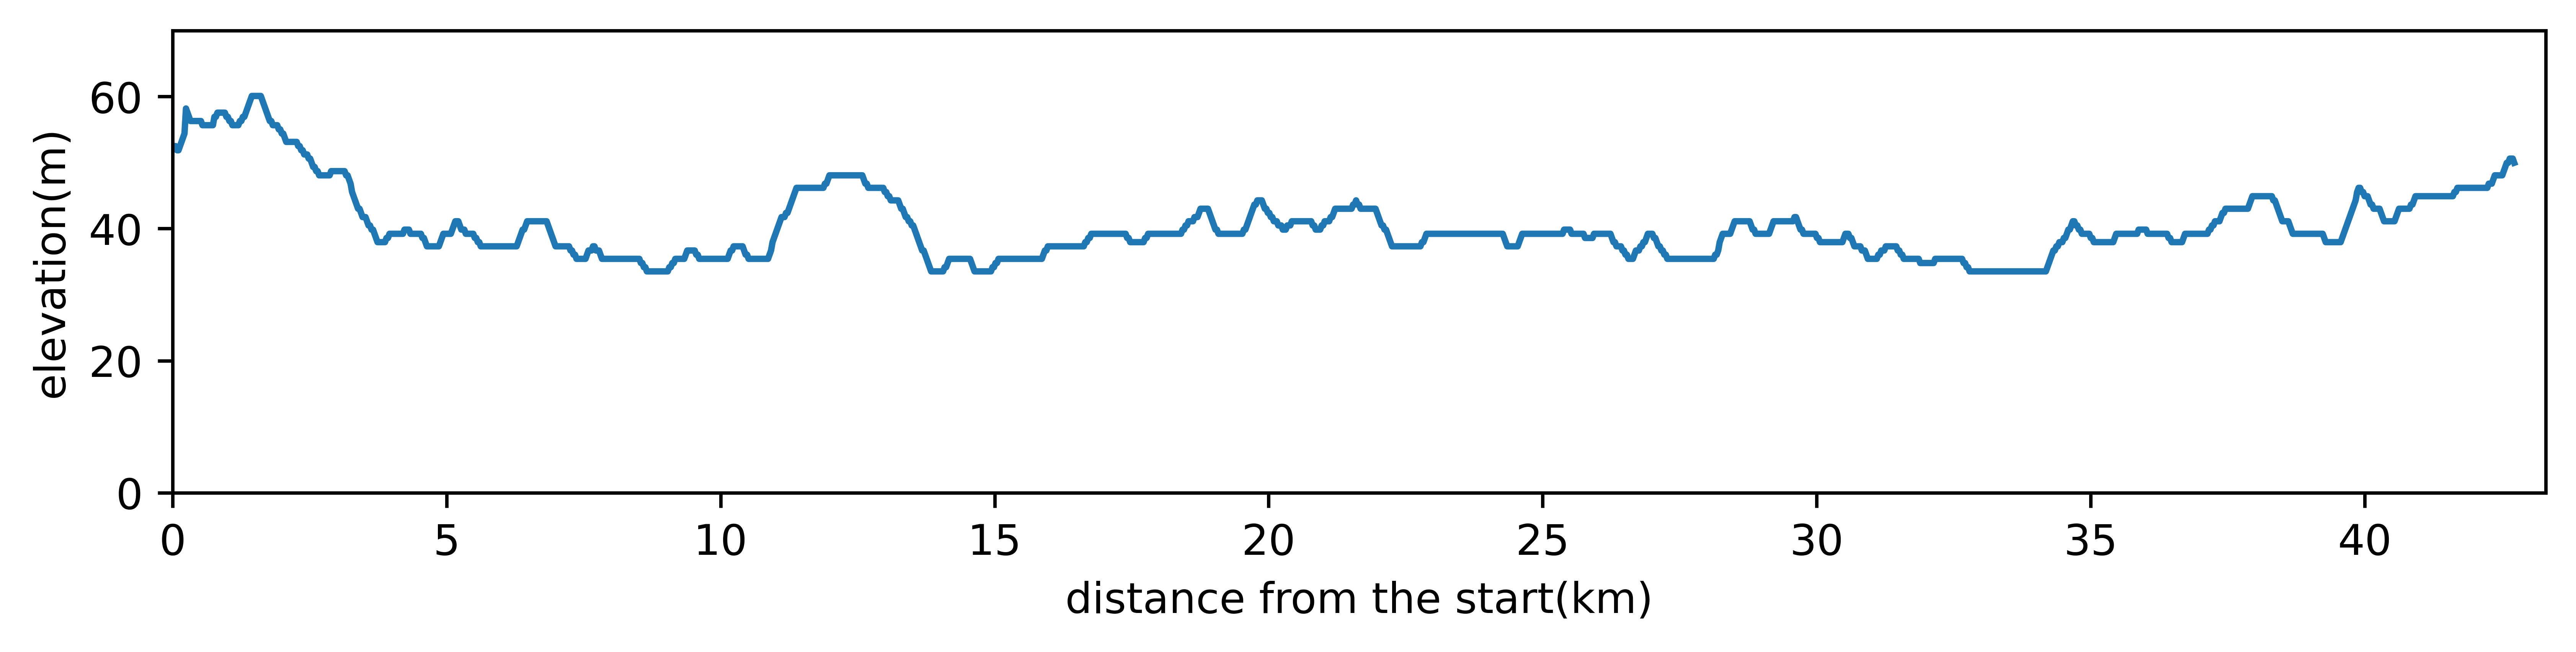
\includegraphics[width=15cm]{7.png}\\
		\small \textit{Fig. 6 and 7  Different trial courses}
	\end{center}	
	Under the requirements in the problem, we later designed our own course. As different types of coursed are needed to respectively justify model A and B, we chose to create a more representative course that meets the \textit{almost linear pattern of slopes} condition as mentioned above. Note that with this pattern, model A actually outperforms model B on both accuracy and calculation speed.Here is our design.

	\begin{center}
		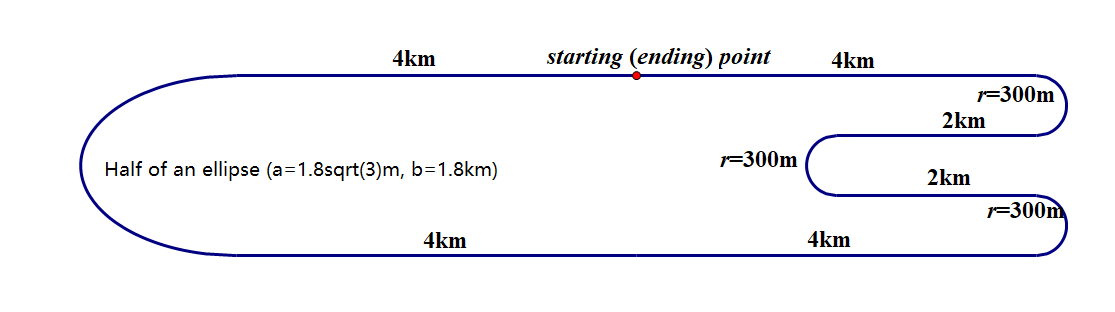
\includegraphics[width=15cm]{8.png}\\
		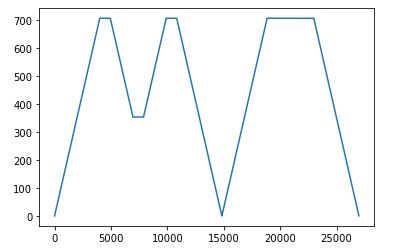
\includegraphics[width=9cm]{9.png}\\
		\small \textit{Fig. 8 and 9  Shape of our "DIY" course }
	\end{center}
	\subsection{Sensitivity Analysis}
	\section{Model C}
	\subsection{Model Overview}
	%In this part, we will build a dynamic sytem based on the relationship between all of these factors. This will hlp us better detect the cyclist's power and energy consumption and provide cyclists with real-time suggestions. Also, we can apply this model to teams who seek to achieve championship.
	After we built a dynamic model to simulate the cyclist's moving pattern, we extend our model to find out the best trategy for a team which is made up of 6 riders. This 
	\subsection{Finding the Best Solution}
	To monitor the cyclist's power curve, we divide the whole process into several "steps", the change of which determines the best solution in the next "step". So we can find that :$v(t)\rightarrow P(t)\rightarrow E(t)\rightarrow \mathrm{next\, decision}$.
	\subsubsection{Fatigue Degree}
	Since our powercurve is a successive function, we identify $f_{\mathrm{fatigue}}$ as the fatifue degree. The bigger $f_{\mathrm{fatigue}}$ is, the more tired the cyclist is. Here's how we define $F_\mathrm{fatigue}$.

	$$E(t)\downarrow\Rightarrow f_{\mathrm{fatigue}}\uparrow$$
    $$\dfrac{\mathrm{d}}{\mathrm{d}t}E(t)\downarrow\Rightarrow f_{\mathrm{fatigue}}\uparrow$$
	$f_\mathrm{fatigue}$ can effectively determine learning rate.
	 The process is shown below.
  	$$\mathrm{Learning\,rate}\xlongequal{\mathrm{def}}L$$
    $$\sigma \left( x \right) =\dfrac{1}{1+e^{-x}}$$
    $\begin{array}{ccc}
		f_\mathrm{fatigue}\left(t\right)&=&\alpha_{\mathrm{fatigue}}\times \mathrm{energy}\:\:\mathrm{proportion}\times \mathrm{how}\:\:\mathrm{tired}\:\:\mathrm{you}\:\:\mathrm{are}\\  
     	\ &=&\alpha_\mathrm{fatigue}\cdot \dfrac{E(t)}{E_\mathrm{total}}\cdot \left( \dfrac{\mathrm{instant}\:\:\mathrm{fatigue}\:\:\mathrm{rate}}{f_\mathrm{fatigue}^{\Theta}}\right)^{-1}\\
    	\ &=&\alpha_{\mathrm{fatigue}}\cdot \dfrac{E\left( t \right)}{E_{\mathrm{total}}}\cdot \dfrac{E\left( t \right) -E_{\mathrm{total}}}{t\cdot \dot{E}\left( t \right)}\\
	\end{array}$

     ($\alpha _{\mathrm{fatigue}}\in \left[ 0,1 \right] $)
     $$\mathrm{standard}\:\:\mathrm{fatigue}\:\:\mathrm{rate}\left( f_{\mathrm{fatigue}}^{\Theta} \right) \xlongequal{\mathrm{def}}\mathrm{average}\:\:\mathrm{fatigue}\:\:\mathrm{rate}=\dfrac{E\left( t \right) -E_{\mathrm{total}}}{t}
      $$
    $$L\left( f_{\mathrm{fatigue}} \right) =1-\underset{\mathrm{the}\:\mathrm{lower}\:\mathrm{bound}\:\mathrm{rate}}{\underbrace{\dfrac{2}{3}}}\sigma \left( \underset{\mathrm{the}\:\mathrm{stretching}\:\mathrm{rate}}{\underbrace{10}}\cdot \left( \underset{\mathrm{translation}}{\underbrace{\dfrac{1}{2}-x}} \right) \right) $$
     \subsubsection{Determining the Ideal Velocity}
	 After we have simulated the cyclist's fatigue degree, we need to find out the best speed which will prevent the cyclist from being exhausted while riding in the maximum speed. In this part, we divide the road into several sections, each of which obatain an ideal velocity. So we define $\vec{c}$ as the cyclist's instantaneous velocity:$\vec{v}=\left( v_1,v_2,...,v_k \right)$ 
	
	 For every section of the road, we have an ideal $\vec{v}^{\Theta}=\left( v_{1}^{\Theta},v_{2}^{\Theta},...,v_{k}^{\Theta} \right) $
	
	 So we can find that:
	$$\Delta ^{\Theta}v=\sqrt{\frac{\sum_{i=1}^k{\left( v_i-v_{i}^{\Theta} \right) ^2}}{k}}\xlongequal{\mathrm{def}}f_{\Delta}\left( \vec{v} \right) $$
	
	After completing all these calculations, we find out the ideal velocity which has the maximum closeness value: $\nabla f_{\Delta}\left( \vec{v} \right) $.


	\section{Strengths and Weaknesses}
	\subsection*{Strengths}
	\begin{itemize}
		\item \textbf{Accuracy}
		
			As relevant constants that appear in our models are not always accessible on the Internet, we adopted the method of fitting data into our model, which derived rather reasonable results. We build a dynamic model to speculate on the cyclist's moving pattern, velocity condition and energy consumption. These two combined, therefore, actually results in a even more accurate model with computational convenience, accuracy and reality.
		\item \textbf{Generality}

			Another part of our model with deep insight is that, instead of attempting to establish a universal model which is able to effectively cope with all types of scenarios, we developed two models (Model A \& B) which respectively excels in patterns with regular slopes and those with irregular ones. 
	\end{itemize}
	\subsection*{Weaknesses}
	\begin{itemize}
		\itembf{NO WEAKNESS HAHAHA}
	\end{itemize}
	\newpage
	\section{Guidance}
	Dear Directeur Sportif:

	Given all the analysis above. We sincerely suggest you to obey the following suggestions:
	\begin{enumerate}
		%\itembf{Every riders should lead the team for a certain amount of time. }

			%This can make sure that the team maintain their maximum speed at a long time. When the head of the team (the leader) is close to exhaustion, he should slow down while the others keep the same so that he will soon become the last one of this team. This will help them build a strong bond against air resistance and strong wind.
		\itembf{}
	\end{enumerate}
	\newpage
	% \setcounter{page}{\wholepages}
	\renewcommand\refname{References}
	\addcontentsline{toc}{section}{References}
	\tolerance=500
	\begin{thebibliography}{100}
		\bibitem{114514} Mathematical Modelling, Qiyuan Kang, Jinxing Xie and Jun Ye
		\bibitem{UCI}2021 Road World Championships Individual Time Trial (Men Elite), UCI,
		
		https://www.flanders2021.com/\_media/races/image\_map/1632122636/fit/1650/0/6/men-elite-individual-time-trial.webp
		\bibitem{france}https://www.topendsports.com/sport/cycling/anthropometry-tourdefrance-tables.htm
		\bibitem{weight}Cycling Physique, science4performance,
		
		https://science4performance.com/2019/09/12/cycling-physique/
		\bibitem{friction}https://zhidao.baidu.com/question/309300297713546924.html
		\bibitem{boltzmann}Boltzmann constant, Dictionaty.com,
		
		https://www.dictionary.com/browse/boltzmann-constant
		\bibitem{time trial record}The time trial speed record, wikipedia,

		https://en.wikipedia.org/wiki/List\_of\_cycling\_records/
	\end{thebibliography} 
\end{document}